\subsubsubsubsection{Lane Decorator}
\begin{figure}[h]
\centering
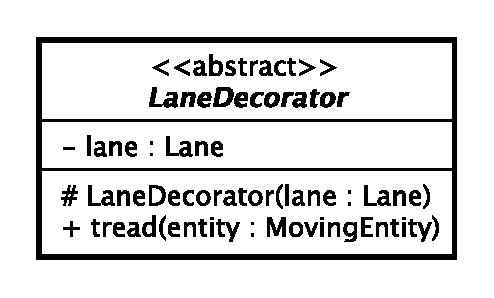
\includegraphics[scale=0.6,keepaspectratio]{images/solution/lane_decorator.eps}
\caption{App::Reactive::LaneDecorator}
\label{fig:sd-app-lane_decorator}
\end{figure}
\FloatBarrier
\begin{itemize}
  \item \textbf{Description} \\
    It represents the abstract decorator which enable to compose togheter several
behaviours on the top of a lane component. 
  \item \textbf{Attribute}
  \begin{itemize}
    \item \texttt{- component: Lane} \\
The lane to decorate.
  \end{itemize}
  \item \textbf{Operation}
   \begin{itemize} 
   \item \texttt{+ LaneDecorator(component: Lane, roadsign: List<RoadSign>)} \\
Creates a lane decorator with a specific lane to decorate with the road signs
in \texttt{roadsign}.
    \item \texttt{+ tread(entity: MovingEntity)} \\
Decorates the standard behaviour of the lane.  
  \end{itemize}
\end{itemize}
